\documentclass{article}
\usepackage{graphicx}


\begin{document}


% Title Page
\title{Data Collection Documentation (Draft 3)}
\author{Steven Deutekom}
\date{July 2019}
\maketitle


% Table of Contents
\newpage
\tableofcontents


% Introduction %%%%%%%%%%%%%%%%%%%%%%%%%%%%%%%%%%%%%%%%%%%%%%%%%%%%%%%%%
\newpage
\section{Introduction}
% What are we doing?
The goal of this project is to collect source code samples from individual authors from various online sources. It requires finding samples that have certain sociolinguistic characteristics such as gender, region, and experience. In addition to sociolinguistic characteristics, it is necessary that the samples are the work of only a single author. Data that meets these needs is being collected and used to create a dataset with information on authors and their source code.

% Why are we doing it?
The collected data will be used for sociolinguistic research into how people use programming languages. Current and future University of Lethbridge students will use this research to learn how sociolinguistic characteristics affect how programmers write code. Previous research was conducted with a small dataset of student programs. This new dataset will contain many samples from a larger set of programmers.

% What is coming in this documents?
The document is broken into three main sections. Each section details one of the sources that was used to collect data. First, the collection methods used to gather source code from GitHub. Then, the methods used to collect source code from Codeforces. Lastly, the methods that were used to add gender data to the samples collected.

Each section introduces the sources and collection methods. Then it discusses the pros and cons of the source. Next an overview of the process of collecting data is given, with diagrams to help visualize it. Following this a more in depth technical examination of the collection process takes place. Finally, some reflection on the source is given (if needed?).


% GitHub %%%%%%%%%%%%%%%%%%%%%%%%%%%%%%%%%%%%%%%%%%%%%%%%%%%%%%%%%%%%%%%
\section{Collecting Source Code From GitHub}


%& Introduction to the sources being used
\subsection{Data Sources}
\subsubsection*{GitHub}
GitHub is one of the largest online code sharing/hosting website on the internet with over 36 million users and over 100 million repositories \cite{WEBSITE:Git1}. It has an API that allows access to information on users, repositories, commits, and more(?Jackies comment was not clear on etc. but I assume it is no good. Whats better?). Source code hosted in public repositories is available for anyone to freely access or use in projects. Data on users, as well as source code is collected from GitHub and added to the database. Two methods are used for this. The first looks at commit data and collects changes to files. The second looks at projects and collects full files of source code. Both support the goal of adding single author source code samples to the database.

\subsubsection*{GhTorrent}
GhTorrent is an offline database of data obtained from the GitHub API \cite{Gousi13}. It contains large quantities of data on GitHub users, projects, commits from as far back as 2012. This data is being collected to support research on software repositories and is available to the public for other research on GitHub. This source is used to collect information on GitHub commits and projects. We use this information to decide what projects and commits to attempt to collect source code samples from GitHub (clumsy). More information is available at http://ghtorrent.org.

\subsubsection*{Google BigQuery}
Google BigQuery is a part of the Google Cloud Platform. It allows the storage and querying of datasets online. These datasets and query results can be connected to other google cloud services and also downloaded. The GhTorrent dataset is accessible on BigQuery. Queries on the GhTorrent dataset are made  using and refined using BigQuery in order to find information on the desired commits and projects.


%% Pros and Cons of each along with steps taken to try and overcome any issues.
\subsection{Pros And Cons}
\subsubsection*{GitHub}
\begin{itemize}
    \item The popularity of GitHub means that there is a large amount of source code and data available. This means one can get a reasonable amount of data on even very specific searches.

    \item It's api is full featured and well documented. It can be used to find any information that is available on the website. Except source code which must be obtained in other ways.
    
    \item The nature of the platform makes all public code freely available for anyone to access within the platform. This is outlined in the GitHub terms of service (reference). However, without and open source license source code is still the sole property of the author and cannot be shared or published without their permission.

    \item GitHub is often used for collaboration. It is not always easy to tell wether source code has a single author, but there are contributor lists and other tools that can help. However, results from the these tools might not be accurate when used on projects that were added to GitHub long after being stated. It is also possible for code in a repository to be taken from a 3rd party source like libraries, extensions, or freely available code samples.

    \item A Rate limit of 5000 calls per hour is imposed on the GitHub API. By collecting the initial data from GhTorrent the number of API calls is reduced. It is not hard for a process to use up this limit in much less time than 1 hour. If a process will use up the limit it is necessary to have it keep track of time and wait for the API to reset every hour.

    \item When collecting code from commits the changes can be scattered around a file. It is not very useful to have 30 lines of code from an author if those 30 lines are not connected to one another. It is possible to identify changes that are part of a newly added file. This ensures that all the changes represent a single piece of code. One of the issues with this is that newly added files are often not complete.
\end{itemize}

\subsubsection*{GhTorrent}
\begin{itemize}
    \item The GhTorrent database is a massive database of GitHub metadata. Accessing GitHub metadata using GhTorrent can make it much easier to know what kind of data is available on GitHub.
    
    \item Because the GhTorrent database is so big it would be difficult to store it locally. Queries on a database of this size would be slow without good hardware. So for most people access must be through another source like Google BigQuery. 
\end{itemize}

\subsubsection*{Google BigQuery}
\begin{itemize}
    \item BigQuery is run with Googles code platform. The hardware used to process queries will run queries on the GhTorrent database much faster than the hardware most people have access to.

    \item Because BigQuery is part of the Google cloud platform it requires a google account to use. There are also limits on the amount of data that can be queried each month and limits on how much data a person can store. It is possible to increase these limits with payment if needed.

    \item BigQuery also has a limit on how many rows of data can be downloaded at once. This can make it more time consuming to download the results of large queries. Details of this process can be found below.
\end{itemize}


%% High level overview of the process w/ diagrams
\subsection{Process Overview}

%%% Ght and BigQuery process
\subsubsection*{GhTorrent and Google BigQuery}
SQL queries are made on the GhTorrent dataset via BigQuery. These queries are refined until the results are satisfactory. Once desired results are obtained they can be saved or downloaded. It is often best to save the results of a large query and then sample it with another query. These sample results can then be split and downloaded. If the results were split they can be recombined before being processed by one of the collection methods for GitHub. See Figure 1.

% Process Diagram
\begin{figure}[t]
    \centering
    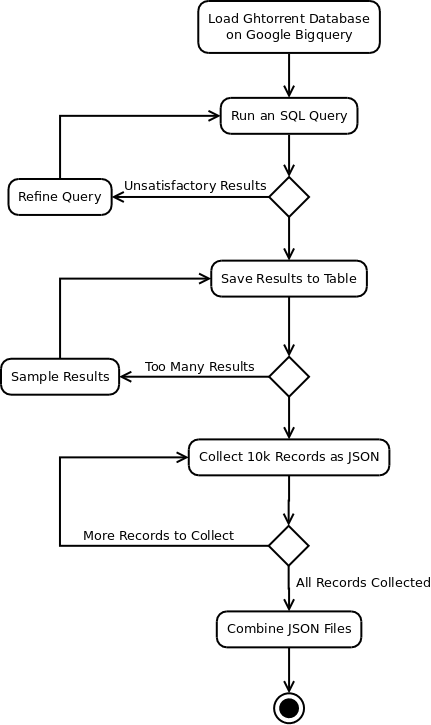
\includegraphics[height=10cm]{diagrams/ght_process.png}
    \caption{Getting Data From GhTorrent}
\end{figure}

%%% Git projects process
\subsubsection*{Collecting Git Projects}
The list of GitHub project data collected from GhTorrent is loaded and each entry is processed. If the project referenced by an entry is valid its repository is cloned locally. Then every valid folder is searched to find valid single author files. All valid files are then processed by having their source code collected and further validated. If the source code is valid it is added, along with user and project information, to the database. Once a project is finished being processed the cloned repository is removed. See Figure 2.

% Process Diagram
\begin{figure}[t]
    \centering
    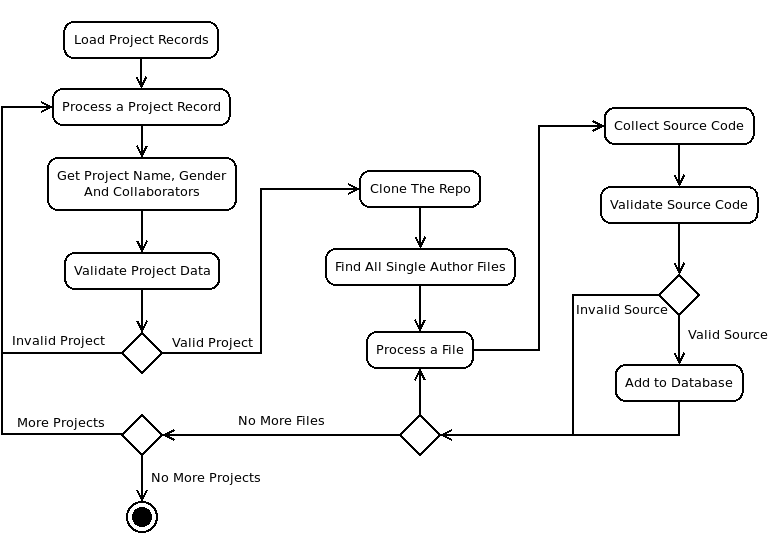
\includegraphics[height=8cm]{diagrams/projects.png}
    \caption{Getting GitHub Project Source Code}
\end{figure}

%%% Git commits process
\subsubsection*{Collecting Git Commits}
The list of GitHub commit data collected from GhTorrent data is loaded and each entry is processed. First the entry's commit information is requested from the GitHub API. If this information is available, all the files that have changes are validated. If a set of changes is valid it is collected and has any extra symbols that were added by GitHub removed. Then the source code is added, along with user, project, and commit information, to the database.  See Figure 3.

% Process Diagram
\begin{figure}[t]
    \centering
    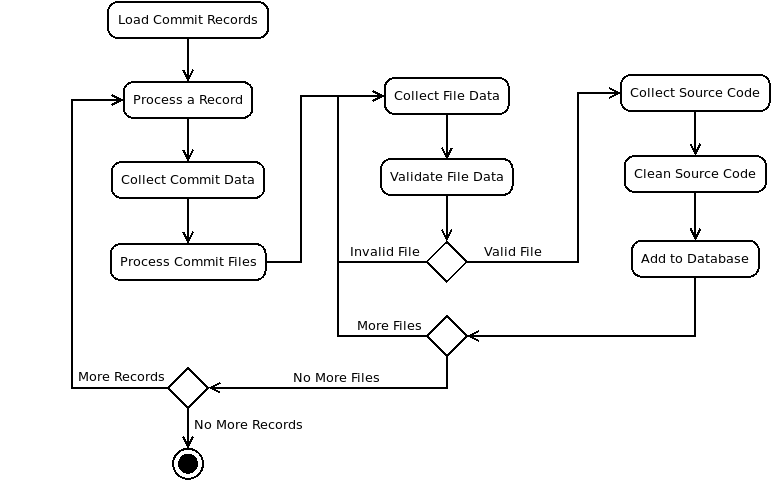
\includegraphics[height=7.5cm]{diagrams/commits.png}
    \caption{Getting GitHub Commit Source Code}
\end{figure}


%% Discussion of each subprocess
\subsection{Process Details}

%%% Ght and BigQuery process
\subsubsection{GhTorrent and Google BigQuery}

\subsubsection*{Process}
The GhTorrent database is accessed via BigQuery at\linebreak
https://bigquery.cloud.google.com/dataset/ghtorrent-bq:ght. From here SQL queries are made on the database to find data for users, projects, and commits. The exact queries depend on which collection method is being used. Both collection methods collect only one programming language at a time, so queries filter out all but the desired language. Since research is being done on region records where country code is NULL are filtered out. These queries run quite quickly and are refined until only the desired results are obtained.

Results are saved to a table in the users personal datasets. A dataset and table can be created to save the results of any query. Though there are only 10GB available in the free tier. Once saved if the results are too big then they are randomly sampled to reduce their size. To build our dataset approximately 150,000 records per programming language were collected. This allowed 6-10,000 users who's combined samples had 300 or more lines of code. When a sample is taken it is saved to a table so it can be downloaded within the constraints of BigQuery.

The final table of results is able to be downloaded with a maximum of 10,000 rows at a time. The table is queried with SQL that allows it to be broken up into pieces that are downloaded as json files. Once each section of 10,000 records has been downloaded as json files they are combined with a script into one or more data files. These resulting data files are formatted so they are can be parsed by Python3's json library and loaded by our scripts.

\subsubsection*{Data}
As described above the data can be downloaded as JSON or CSV. When downloaded as JSON each record is a JSON object that has each column name from the query associated with the value. These are contained each on their own line, but are not in a list, which is why they must be pre-processed and combined. Once processed each record will be an entry in a list and can be looped over in a program. It will be possible to access each value in a record by a key corresponding to the column name from the SQL queries made on BigQuery. Some fields may be null.

%%% Git projects process
\subsubsection{Collecting Git Projects}
The main aim of collecting Source code from projects is to get a large number of samples for an author. The hope is that these samples are working code and that they can be attributed to only the one author. To do this repositories can be checked to make sure they only have one contributor and files checked to make sure only one contributor has written code in them.

\subsubsection*{Process}
First the GhTorrent data is loaded. Then For each one of the entries some data is added to the project. The first is a full name. This is collected by using the GitHub API to find user information and collect a full name. If there is a full name it will be split to find the first name and then passed to a gender checking function. The result of the gender check will also be added to the record. If a name and gender were successfully added to the project data. Then the GitHub api will be queried for the project to find the number of contributors. If the number of contributors is no more than 1 the project will be processed further.

Next the script clones the project repository into a temporary directory. Once downloaded the directory tree is searched. Files and folders that should not be processed can be specified in the configuration for the scripts. If examined files are not in the excluded list they are checked to make sure they have an extension that matches the programming language of interest. All valid files are checked with git blame to determine if more than one author worked on them. Since the user information gathered is for the repository owner the file author must also match the repository owner. When all files are checked all valid ones are returned as a list of filenames.

Each file is then opened and it's source code is collected. The number of lines in the file is collected and checked to see if it is in the range [10, 1000]. If the source is valid then the source and file information are added along with relevant user and project information to the database. Once all the filenames have been processed the next project is processed.

The process continues until all projects in the data file are processed or a given limit for number of projects to process is reached. When finished some details of the process are printed to the console.

\subsubsection*{Data}
Information on the user is collected for GitHub login, full name, country code, and gender. These categories must have values in order for a project to be processed. There is also some other user information like state, city, location, time created, type, and company. This data is allowed to be NULL. Information on the project like it's name, it's api url, it's creation time, and it's primary programming language are saved as well. These always guaranteed to be included in records in the GhTorrent database. The file has it's filename/path, number of lines, and the source code added to the database as well. These are all added to the information saved in the database by the script.

\subsubsection*{Technical Issues}
Because so many external services are connected to during this process connection issues can interrupt the scripts. These are not always easy to handle gracefully and as a result it may not be possible to automate collection without occasionally having to restart the scripts.

Because projects are being cloned if a project is really large it can take a long time. Often projects of this size are not single contributors, but they occasionally don't show up like this when they are validated. If a project has many assets like photos or videos it can really increase the download times. This may not be an issue with a fast computer and connection, but it can affect collection.


%%% Git commits process
\subsubsection{Collecting Git Commits}
The second method which is used to collect source code samples involves using GitHub commits. (needs more or should be cut?)

\subsubsection*{Process}
The process starts the same as the GitHub projects process. It loads a data file of commit info and processes each entry. Each commit first has the commit data gathered from the GitHub API. This data contains the changes that were made to each file that was included in the commit.

The information for each set of changes to a file is validated. These changes must represent a file that was newly added with the commit. They must also be at least 10 lines long. Files must also end in an extension for the programming language of interest. The files that meet these criteria have their source code gathered.

Before a file can be added to the database its source code must be cleaned. The commit stores file changes with a header that has information on the number of changes which has to be removed. Changes for newly added files have a + sign at the beginning of each line. These are also removed before continuing.

Once the source is cleaned it is added along with the user, project, and commit info to the database. Then all the remaining files are processed before moving onto another commit.

The process continues until all commits in the data file are processed or a given limit for number of commits to process is reached. When finished some details of the process are printed to the console.

\subsubsection*{Data}
The data contains the same user and project information as the projects data. It adds some information on the commit. The commit SHA is a unique id that is assigned to a commit on GitHub, and the time the commit was created is also added. The file lines are renamed to file changes as they are a little different (are they?).

Each file that was changed has a list of lines that were altered by an author along with a + or - to indicate if the line was added to or removed. each file also indicates weather it was added in full with this commit or an existing file that was modified. In order to get changes that are not distributed at random points through a file only files that were newly added with the commit are kept


% Codeforces %%%%%%%%%%%%%%%%%%%%%%%%%%%%%%%%%%%%%%%%%%%%%%%%%%%%%%%%%%%
\section{Collecting Source Code From Codeforces}


%% Introduction to the source being used %%
\subsection{Sources}
Codeforces is a website that hosts programming contests. The operators of the site describe it as a social network for people interested in contest programming and as a platform for hosting programming contests (cite their website). Users of the site have access to past contests as well and are able to write and submit solutions to current and past contests. These solutions are available on the user's profile. The website has an API that can be used to collect user and submission information, but does not facilitate gathering source code for solutions. It is one of the more popular sites available for contest programming and hosts many contests. As of May 2019 there were over 180k users that had participated in at least one ranked contest.

%% Pros and cons of collecting from codeforces along with steps taken to try and overcome any issues. %%
\subsection{Pros And Cons}
\begin{itemize}
    \item Making the source code of user's solutions available for anyone to view is not common with programming contest websites. This makes Codeforces a valuable resource for this kind of programming.
    
    \item Codeforces is very popular among users in Eastern Europe and parts of Asia. There is more regional diversity than sites like GitHub that are more popular in North America.
    
    \item Users that participate in ranked contests have a rating that is adjusted based on their performance. This makes it possible to get an idea of a programmer's skill and experience.
    
    \item Users that choose to enter one have a first name. This makes it easier to use the first name to find gender of the programmer. This name is included in the list of users that is used to collect submissions. This allows the user list to be preprocessed for gender before it is run through a script to collect submissions.

    \item The way that solutions are stored makes it more difficult to automate their collection. The source code is stored in popups on the users submission page. So in order to access this code the popups must be opened first. Submissions are supposed to have links to individual pages to view the source code as well, but these links can very be unreliable.

    \item Because there is not API to get submission code it must be scraped from the html. This is not too difficult, however, any changes to the website that alter the html can require adjusting the scripts that collect the data.

    \item Contest programming has very different purposes than more general kinds of programming. Its domain specific nature will be reflected in the source code samples form Codeforces. However, this means that the coders are less likely to adhere to any best practices or style guidelines. There may be even more variation in the coding style between authors. It may just require a different kind of feature selection than other kinds of programming.

    \item The ratio of men to women is quite skewed. It is not easy to find large numbers of female candidates from every country.
\end{itemize}

%% High level overview of the process %%
\subsection{Process Overview}
First a list of users is filtered and gender information is gathered for all users it is possible. Only users with country and gender information are kept. Once a new user list is obtained sections of it are pulled out for specific countries and genders. Each entry of these smaller list is processed. For each entry submission information is collected for the user. If a submission is valid then an attempt is made to collect its source code. If the source code can be collected it is added, along with user information, to the database.

\begin{figure}[!h]
    \centering
    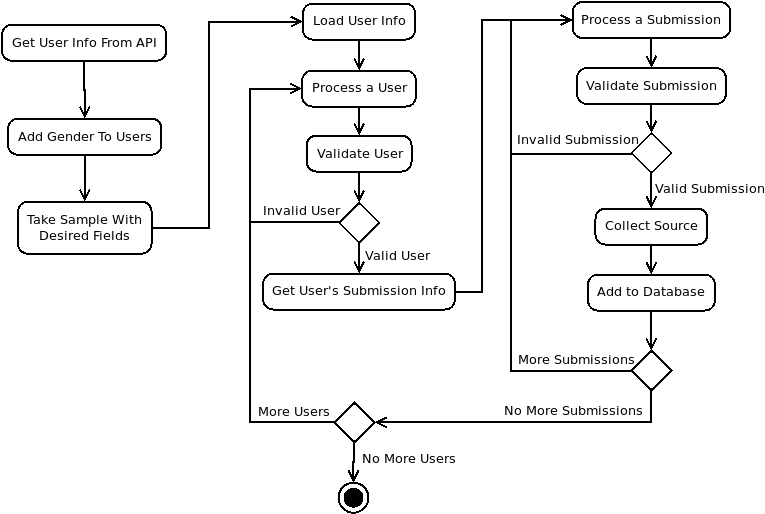
\includegraphics[height=8cm]{diagrams/cf_process.png}
    \caption{Getting Data From Codeforces}
\end{figure}


%% Discussion of each subprocess with technical details, the data collected, and the technical issues %%
\subsection{Process Details}
There are Two ways to collect the code. The most reliable is to use the selenium web driver to open the users submission page and open and close popups to collect the code. The other way is to follow direct links to a page that has the source code on it. As mentioned above the second way is not always available so it is used as a fallback if the no source is available from the selenium method.

\subsubsection*{Process}
First the list of users is loaded by the script. Because the users are preprocessed to filter out valid ones there is no need to validate the users as they are processed. For every user first information on their submissions is collected. When using selenium only the most recent 50 are gathered because the submissions page has 50 submissions per page. Before processing the submission list the database is queried to get the problem names of all submission that the current user has in the database. These are added to a set that keeps track of problems so that code is not collected more than once for a problem. The variations in submissions for the same problem are often quite small, especially if they are both accepted solutions.

Each submission is checked to see if it is valid. It is checked to make sure that it was not a team submission, that it was an accepted submission, and that it is not a problem previously collected for the current user.

There are 2 different ways to collect the submissions source code. With selenium this involves clicking the link to a submission. All submissions are stored with a unique id so it is easy to find the link using a submission id and searching the pages html. Once this link is clicked a popup will open that contains information on the submission including it's source code. When this popup is opened it's contents are now part of the pages html so it is scraped to obtain the source code. After this the popup is closed.

If selenium is not used, or for some reason selenium fails to find any source code a link is assembled using the user and submission information. This link leads to a standalone page for the submission source code. Since this page is not always available, which is why this process is used as a backup to the selenium process. The html for this page collected and it is scraped to obtain the source code.

Once the source code is collected it is added along with user and submission information to the database. Then each remaining submission is processed. When all 50 submissions are processed or 50 submissions have been collected for the user next user is processed.

The process continues until all users in the data file are processed or a given limit for number of users to process is reached. When finished some details of the process are printed to the console.

\subsubsection*{Data}
The data that is collected contains two different kinds of information. The first is user information. Some information is always present and some is filtered if it is not. Always present information for a user is a unique codeforces handle that identifies a user on the website, a ranking that is a string identifying how well rated a user is, a rating which is a number between 0 and 4000 (actual?) that is adjusted based on solutions and failures to ranked problems in contests (are you sure) it works similar to rating systems in chess, and a registration time. Some information is optional like first and last name, country, and organization. If a user does not have a first name gender cannot be found so users without first name are not used. Also, users without country are not used either as this is an important sociolinguistic feature. If a user has a first name, but gender cannot be collected for that name then that user is also not used.

The second kind of information is for the submission. This includes a submission id, a problem name, a programming language, and submission time. It also includes problem difficulty, but this is not always available and participant type (which I am not sure I really know what that is). If source code is gathered for the submission it is saved as a string of the program text. All of these things are added to the database for each submission that is collected. The data that is collected from the api is in json format and is loaded and parsed to find the appropriate information for querying the api for the user submissions and for validating and collecting submissions. There are more fields in the API return than are saved with a submission and they an be viewed on the Codeforces website API reference.

\subsubsection*{Technical Issues}
There are some technical issues with using selenium. Since the program physically loads each page and interacts with it the program must pause to wait for the pages to fully load before it continues. This means that there are some sleeps in the code for a couple seconds before scraping a popup and after closing one and clicking the next submission. These sleeps are as short as possible, but they do slow the collection down. However, as the selenium usually gets all code that is available it is preferable to running the links script which often will get nothing for a large period of time as links are unavailable. Also, because the codeforces web page is loaded it requires loading all of the extra information that is required to open the whole webpage. This often means waiting for certain services to be connected to or loaded. Some of them can fail to load for many minutes. To get around this the script will wait for only 30 seconds and then refresh the page. Often this will fix issues with loading all services. It can reduce the wait time when switching to the submission page of a new user to a couple minutes or less. Also, sometimes the popup cannot be found to close by the selenium script and it is necessary to refresh the page. Also, if all methods of collecting source code are unsuccessful the script will wait for 30 seconds to hope that the website services are working again. This helps to ensure that all code for a user is collected that can be from their first 50 submissions. All of these issues are handled by the script so that it can be automated, However, there are still occasionally errors when interacting with systems like websites and databases that cannot be easily recovered from. Because of this it is not always easy to leave the script running unattended without checking in on it from time to time.

The main issue not using selenium is link availability. The links seem to stop being available after a around 20 of them are accessed. It can take some time for them to start being accessible again. This means that many submissions for a user could go uncollected even though there is code available for them. It could be possible to put in some sleeps to wait once code is no longer being found so that fewer submissions are skipped, but the wait here can be 10min or more and be encountered after only a few minutes. However, this method is much more stable in that it will often run for a long time without error. So if the other method were to be having issues running for long enough it might be just as easy to let the link method sleep or even just miss some samples while looking for code because it might run for days unattended. (I am not sure that this claim is still valid after adjusting the code)

% Gender Labeling %%%%%%%%%%%%%%%%%%%%%%%%%%%%%%%%%%%%%%%%%%%%%%%%%%%%%%
\section{Adding Gender Labels}
One of the sociolinguistic features that is important to the project is Gender. Unfortunately, gender is available for authors on GitHub or Codeforces. Since it cannot be collected along with author information gender must be obtained in other ways. This can be done using an authors first name. There are a number of websites and APIs available that offer gender data for first names. All the gender information for authors in the dataset were gathered in this way.

%% Introduction to the sources being used %%
\subsection{Sources}
There are several websites and APIs for adding gender for first names. They include gender-api.com, genderize.io, namsor.com, and nameapi.org. This project primarily used genderize.io because it is free and allows 1000 name lookups per day. In addition to this a table was kept in the database to store the names that were already known. The service offers a 'male', 'female', or 'unknown' verdict when given a name. It also gives a probability that a result is correct (from sample?). In addition it is possible to pass a country code to along with the name to obtain results that are more specific? The other APIs all offer similar services, but they all require monthly payment for more than a small number of name guesses.

%% Discussion of the pros and cons and difficulties along with steps taken to try and overcome any issues. %%
\subsection{Pros And Cons}
\begin{itemize}
    \item This is really the only way to add gender labels to programmers without being able to ask them directly. Asking them directly would be a significant undertaking and most would be unlikely to respond.
    
    \item With several decent sources available for this kind of labeling it is possible to confirm results. If one has selected a portion of the dataset that meets their needs it would be possible to re-run the authors names through all the services and filter out any users that could not be agreed upon. This could improve the accuracy of the labels. Doing this with a smaller dataset would also reduce the cost of using services that require payment. Also, there are many names that are more common so the number of names needed will always be less than the number of authors in a dataset. This will further reduce the number of names to label and should mean that reasonable accuracy can be obtained for many common names.

    \item Inferring gender from names is not an easy task (some examples and sources). It is also not always very clear how a service is determining the gender \cite{Santamaria2018}. So this is immediately a problem. The probability given can help to determine the likelihood of results being correct, but it still is only as good as the service. There are some stats given by Santamaria \cite{Santamaria2018} that comment on the accuracy of the above 4 services.

    \item Aside from the accuracy of these methods being suspect, the major con is that for the most part they are paid services. Some of them do offer free limits, but only genderize is really worth it for any larger needs, and even then only with an offline backup of already labeled names. The good news is that there are many people sharing a small number of names, so a large number of samples can be labeled with a small database.

    \item People are not always truthful with their names on these profiles, sometimes they do not even give a name. As a result there are fewer samples to work with if gender is desired. If country is going to be used to add accuracy to the label then it lowers the number of samples available further.

    \item All services are less effective at labeling Asian names \cite{Santamaria2018}. This can present a problem for datasets that are using large numbers of samples from Asian countries.

    \item The number of samples can be low for a name so even if the probability is high it may not be accurate.

    \item The names collected show a much less accurate probability for female names. Most male names are classed as 0.9-1.0 and more female names fall into this category, but in some cases at most half of the names are in the 0.9-1.0 category. This suggests that there are some issues with classifying female names properly. Wether it is that more female names are unisex or that there are low samples for them is unknown (to me. Could use a table?).
    
    \item These methods of gender labeling are firmly rooted in the gender binary. The gender labels of names will be more likely to be connected to cultural norms and biological sex and may not accurately represent the individual' gender.
\end{itemize}


%% Overview of the process %%
\subsection{Process Details}
\subsubsection*{Process}
The process used for collecting gender for names is relatively simple. Given a name the database is checked to see if it has the name already. If the name is not in the database it is looked up with the genderize.io API. If the API returns a result that result is added with the name to the database. If the API limit has been reached then a appropriate (what?) response is given. The scripts all have options (Do they?) to save results for later processing if gender cannot be determined. If there name is able to be labeled then the label and the probability are returned.

The labels added to the scripts do not use country codes. As stated above it will be desireable to re-label the names on samples that are used by submitting the names and countries again to other APIs to see if results can be confirmed or refined. Because this will be done after it is likely that some authors will have been missed because they had unknown genders and so they were not added to the dataset. This may throw off the statistic of the samples a bit. The most important thing is to have enough good samples with reliable gender labels to use in experiments, so loosing a few users is acceptable. Better to have less data that is high quality than to have more data that is lower quality.

\subsubsection*{Data}
The data consists of just the gender and the probability the gender label is correct. The gender is a string 'male', 'female', or 'unknown' (Other APIs give different results). The probability is a float between 0.0 and 1.0. The Case of a name is ignored (is it?). There is also a 'count' field that is returned that is described as 'the number of entries examined to calculate the result' (cite). and if country code is given the country code is also part of the response. Also the name is part of the response.


% Database ???? %%%%%%%%%%%%%%%%%%%%%%%%%%%%%%%%%%%%%%%%%%%%%%%%%%%%%%%%

% Conclusion %%%%%%%%%%%%%%%%%%%%%%%%%%%%%%%%%%%%%%%%%%%%%%%%%%%%%%%%%%%
\section{Conclusions}
% Comment on the successes and failures?
% Future improvements or additions
Reserved for when I am closer to finished and can discuss the results with everyone else. Perhaps identify some future tasks or current deficiencies.


\newpage

\bibliography{technical_report}
\bibliographystyle{apalike}

\end{document}